\chapter{Analysis, Design and Test}
This chapter describes how the tool has been implemented using Python (version 3.4) as the programming language. The input to the tool are given as JavaScript Object Notation (\emph{JSON}) files and the tool also outputs a JSON file.

\section{Design}
The implementation has been done by dividing responsibilities into separate modules and classes. In total, the tool consists of 8 modules and 27 classes. To explain how the tool is implemented \autoref{fig:class-diagram} shows a high level class diagram. \autoref{fig:class-diagram} does not show all the classes to simplify the class diagram. Furthermore not all methods and attributes in the classes are shown.

\begin{figure}
\centering
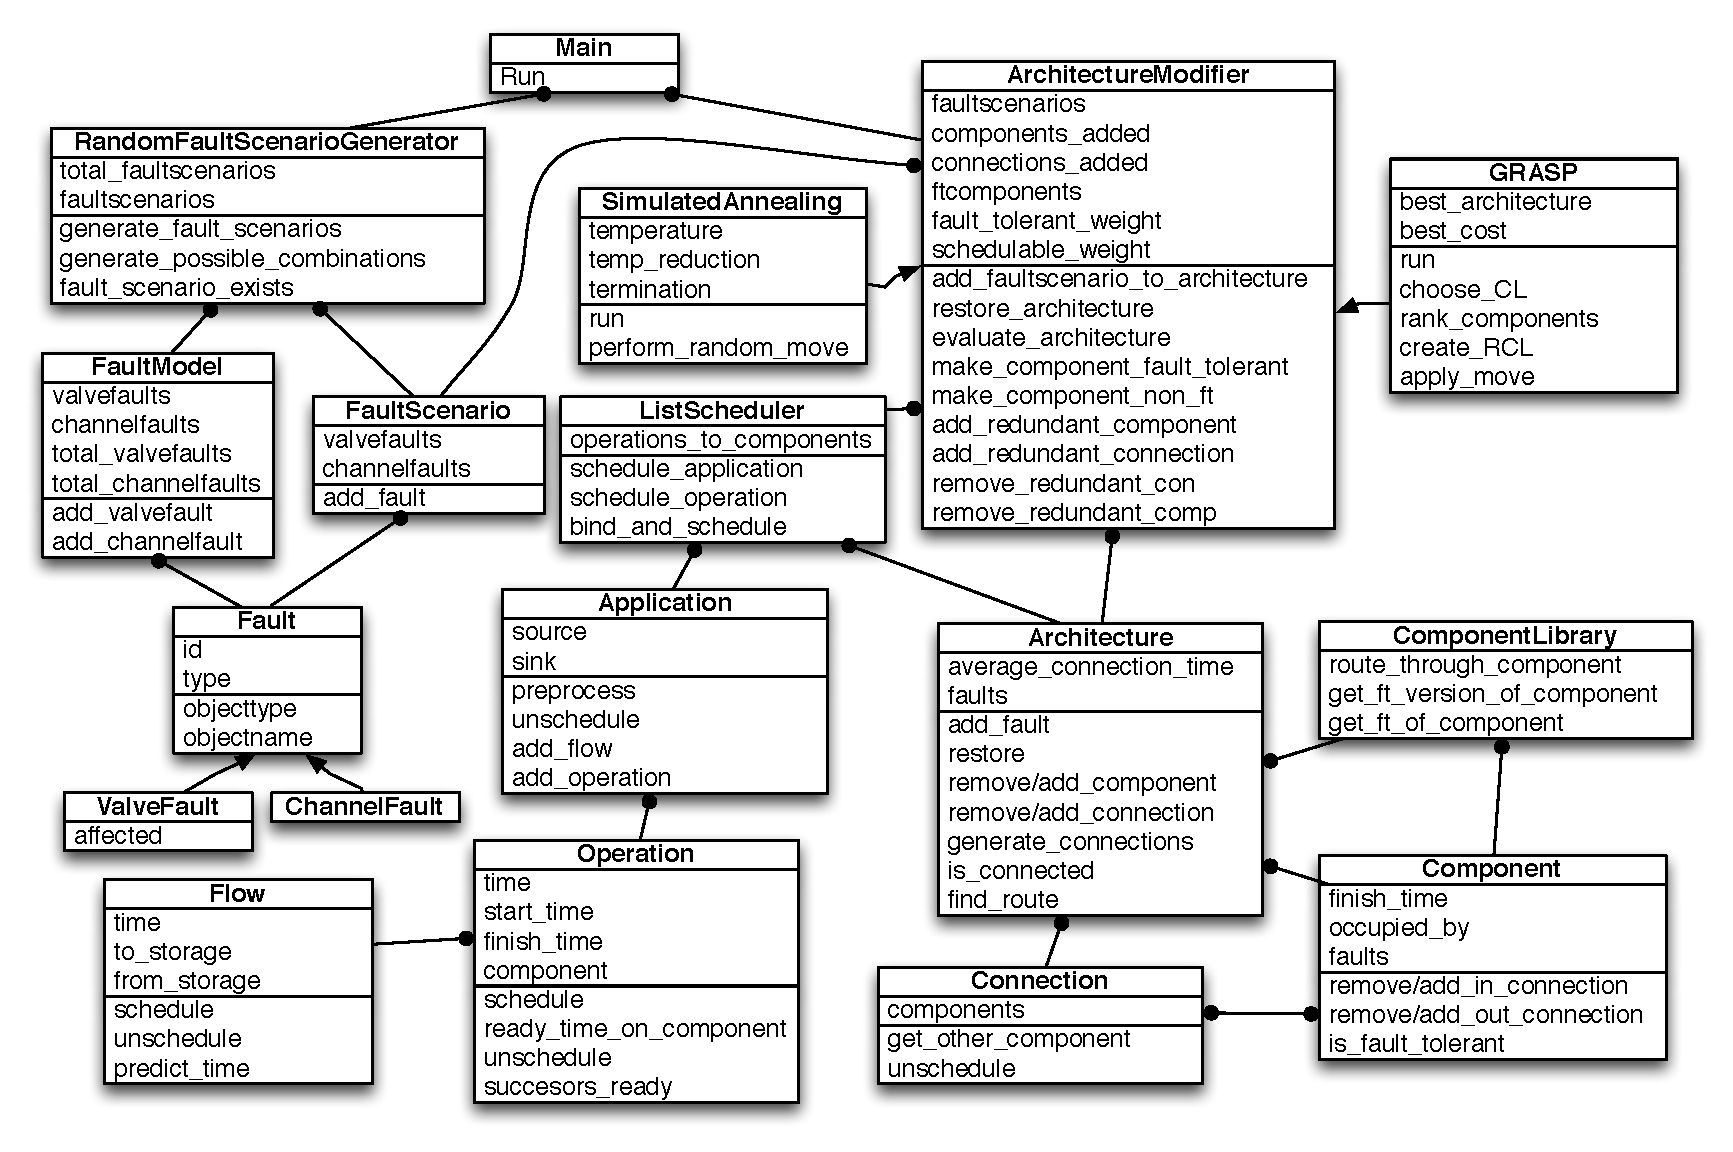
\includegraphics[scale=0.425]{figures/ClassDiagram.pdf}
\caption[Class diagram of the implementation]{Class diagram of the implementation}
\label{fig:class-diagram}
\end{figure}

In the following sections each module will be described and each class within the module will be clarified.

\subsection{Architecture}
The architecture module contains the classes for the architecture model, components, connections, component library and routes. The \emph{Architecture} class implements the architecture model and it has the responsibility of adding and removal of components and connections, finding routes for the fluid and generating the effects of faults. When finding routes between components, the architecture considers the effects of valve faults on switches, i.e. it might only be able to use certain connections if the valve is faulty. Similarly, the route search also considers blocked channels. Furthermore, it contains methods to add faults and restore from faults. The architecture uses the \emph{Component}, \emph{Connection} and \emph{ComponentLibrary} classes. The component class specify the type of the component, the in and out connections it has and furthermore it has scheduling related specifications. The connection class specify a simple graph edge and knows the two component it connects and it has details about scheduling. The reasoning behind components and connections having details about the scheduling is that it simplifies the scheduler, and unscheduling is also simple as it is just the resetting of used attributes. The component library has all the possible components and it keeps track of which components have and do not have fault-tolerance, the fault-tolerance of the components and which components they are the fault-tolerant version of.

\subsection{Fault Model}
The fault model module contains classes for the fault model, the faults, fault scenarios and the random generation of fault scenarios. The \emph{FaultModel} class is simple as it contains two sets which distinguish channel and valve faults, the maximum number of valve faults and the maximum number of channel faults. \emph{Fault} is a superclass which has two subclasses \emph{ValveFault} and \emph{ChannelFault}. The fault class specifies the object type the fault affects, either component or connection, and the name of component or connection, where the names of components and connections are specified in the JSON file for the architecture. The \emph{FaultScenario} class contains a set of valve faults and a set of channel faults. The \emph{RandomFaultScenarioGenerator} class implements the fault scenario generation algorithm described in detail in \autoref{sec:fs-gen}.

\subsection{Application}
The application module implements the application graph, the operations and the flows (edges) in the application graph. The \emph{Application} class contains a preprocess method for preprocessing the application graph and functionality to unschedule the application such it can be rescheduled and thereby a new schedule in the objective function can be found. The preprocessing consists of adding a source and a sink as operations to the graph. The source is added such that all the input operations depend on the source and the sink is added such that the sink depend on all the output operations. The \emph{Operation} class represent operations in the application graph. The class implements methods to find the ready time on specific components, which considers the routing time and constraints. The \emph{Flow} class model the dependencies (edges) in the application graph. The class implements methods to schedule the flows to storage and from storage if needed when scheduling, and they can easily be unscheduled.

\subsection{Parsing}
The parsing module contains all the parsers for the JSON files. The module contains a superclass named \emph{Parser}. In total, the tool receives 5 files and there is a class to parse each type of file, where all are subclasses of Parser. The \emph{ArchitectureParser} is responsible for parsing the netlist from the JSON file and create an object of the architecture class. Similarly, \emph{ApplicationParser}, \emph{ComponentLibraryParser}, \emph{FaultModelParser}, and \emph{ConfigParser} create the application graph, component library, fault model and the config data, respectively. The config data specifies the average routing latency, application deadline, number of fault scenarios, which algorithm to use and the algorithm specific details.

\subsection{Scheduling}
The scheduling module implements a superclass \emph{Scheduler} such that it is easily extendable to implement more schedulers if more schedulers are needed. The \emph{ListScheduler} class is a subclass of Scheduler. The ListScheduler class implements the List Scheduling algorithm which is described in detail in \autoref{sec:list-scheduling}.

\subsection{Architecture Modifier}
The architecture modifier module implements the design transformations, architecture evaluation, SA and GRASP. It has three classes \emph{ArchitectureModifier}, \emph{SimulatedAnnealing} and \emph{GRASP}. The ArchitectureModifier is a superclass which implements the design transformations, evaluates the architecture using the fault scenarios and keeps track of the added components, connections and fault-tolerant components converted. The moves are described in detail in \autoref{sec:moves}. Converting a component to fault-tolerant is simple as the type of the component just needs to be changed to the fault-tolerant type. Similar is the case, when converting it back to its regular version. When adding a connection, we just need to consider that the components do not get more incoming or outgoing channels than they are able to handle. Recall that a switch can only consist of four valves (channels) which also means that, e.g. a mixer cannot have more than two incoming and outgoing channels. Removing a connection is also simple as we keep track of the connections, we add to architecture and only redundant connections can be removed. Adding a redundant component however adds more complexity. The move is implemented such that the incoming and outgoing connections are always from / to switches. Consider the situation where all switches already have the maximum allowed channels, then two connections between two switches has to be modified to add a switch between them such that we can add the new component. Removing a redundant component therefore has to take this into consideration. It is implemented such that if a component has added switches to the architecture and we want to remove it, then it also removes the switches if, and only if, the switches do not have a connection to other components than the one, we wish to remove, and the switches from the connection, we modified. If the switches have connections to other components, they are kept in the architecture and added to the list of added components such that it is possible to remove. If it is removed later on, it will add the connection that we modified to the architecture.

Simulated Annealing and GRASP are subclasses of the ArchitectureModifier class as they use the moves and the architecture evaluation of their superclass. SA and GRASP are explained in detail in \autoref{sec:sa} and \autoref{sec:grasp}, respectively. The ArchitectureModifier superclass makes it easy to extend the tool with more algorithms to produce a fault-tolerant netlist that use the same moves and evaluation method.

\subsection{Serializing}
The serializing module contains two classes, a superclass \emph{Serializer} and a subclass \emph{NetlistSerializer}. This is to output the JSON file specifying the fault-tolerant netlist produced from this tool. The superclass is created such that it is easy to extend with more serializers, e.g. a serializer for applications. 

\subsection{Run}
The run module is the main file for running the program. It takes the command line input which is the JSON files specifying the initial netlist, application, fault model and config file.

\section{Testing}
The tool has been tested in an incremental manner as the different aspects was implemented. The scheduling was one of the first functionalities that was implemented. It was tested on different architectures with the associated application models using the architectures and applications provided by the work of \cite{wajid} and \cite{michael}. The example in \autoref{sec:prob-for} has been used as the key example for all steps in the implementation process. When the logic to generate faults was implemented, this example was used to test that the architecture responded in the correct way when finding routes and determining the connectivity of the architecture. Furthermore, we also tested how the faults affected the scheduling by affecting it both with faults that would make it impossible to schedule the application and contrary with faults where scheduling would still be possible. When it was determined that the effects of the faults were implemented correct, the moves were implemented. The moves were tested in different stages. First they were tested to see if when applied to an architecture the outcome was appropriate. When that test succeeded, it was then tested by affecting the architecture with faults that would affect connectivity and scheduling. Redundancy was then added to compensate for the faults and the outcome should be that the connectivity test and the scheduling would pass. After successfully implementing the moves, SA was implemented to use these moves and it was tested many times using the key example from \autoref{sec:prob-for} to make sure that the moves and their counter-moves were acting correctly when applied many times. GRASP was then implemented and tested similarly to SA.

\section{Summary}
This chapter outlines how the tool was implemented using a class diagram and explaining the different modules and classes. The implementation has been done such that it is easy to extend with new algorithms that will use the same objective function and moves as SA and GRASP and implement new scheduling algorithms. Similarly, every aspect of the tool is implemented. The testing was done incrementally where examples have been used to test every aspect of the tool.